\documentclass[a4paper,11pt,utf8]{scrartcl}

\usepackage[ngerman]{babel}
\usepackage[utf8]{inputenc}
\usepackage[a4paper, left=2cm, right=2cm, top=1.5cm, bottom=1.5cm]{geometry}
\usepackage{graphicx}
\usepackage{stmaryrd}
\usepackage{listings}
\usepackage{amsmath}
\usepackage[hidelinks]{hyperref}
\usepackage[onehalfspacing]{setspace}

\setlength{\headsep}{.5cm}

\begin{document}

\pagestyle{empty}

% Titlepage
\noindent
Praktikum: Big Data \hfill Klemens Schölhorn, Sebastian Lange, Simon Hüning \hfill 04.02.2016\vspace{-.4cm}\\
\begin{center}
\huge\textsf{Lösungsskizze}\vspace{.1cm}\\
\large Zitierungsanalyse auf den Daten der DBLP unter Verwendung von Apache Kylin
\end{center}

\section*{Einleitung}

Die ersten zwei Abschnitte beschreiben die Server Konfiguration und die Vorüberlegungen zum Datenbank-Schema. Die darauf folgenden Abschnitte befassen sich mit der Umsetzung der Aufgaben sowie dabei auftretenden Problemen und in Folge dessen getroffenen Entscheidungen. Das Dokument soll die durchgeführten Arbeiten erläutern und bestimmte Entscheidungen während des Projektverlaufs nachvollziehbar machen. Es stellt \textbf{keine} detaillierte Installationsanleitung dar. Diese befindet sich im Wurzelverzeichnis des zum Projekt angelegten Repository.


\section{Server}

\subsection{Software}

Auf dem für das Praktikum zur Verfügung gestellten Rechner \texttt{wdi06} wurde basierend auf dem im installierten Ubuntu 14.04 LTS enthaltenen opendjk-7 folgende Software installiert:

\begin{itemize}
    \item Hadoop (HDFS): 2.7.1
    \item HBase: 0.98.15
    \item Hive: 0.14.0
    \item Kylin: 1.1
    \item Flink 0.10.1
\end{itemize}

\noindent
Es konnten aufgrund von Beschränkungen von Kylin\footnote{\url{http://kylin.incubator.apache.org/docs/install/index.html}} keine aktuellen Versionen von HBase und Hive verwendet werden. Es existiert zwar eine Version von Kylin für HBase 1.1.3, letzteres wurde jedoch noch nicht offiziell veröffentlicht.

\subsection{Einrichtung}

Die Hadoop-Umgebung wurde im pseudo-verteilten Modus installiert, d.\,h. es werden die gleichen Knoten wie in einer verteilten Umgebung verwendet, jedoch alle auf einer physischen Maschine und nur jeweils eine Instanz pro Knotentyp.

Die Installation erfolgte ohne root-Rechte in einem Benutzerverzeichnis durch Setzen der benötigten Umgebungsvariablen (\texttt{HADOOP\_HOME}, \texttt{HBASE\_HOME}, $\dots$). Dabei wurde weitgehend auf die Standard-Konfiguration gesetzt und nur die minimal benötigte Konfiguration vorgenommen.\footnote{Details dazu finden sich im Installationsprotokoll im privaten Repository: \texttt{Installation.txt}}

Da die meisten Dienste standardmäßig an allen Adressen (und damit auch der öffentlichen Adresse) lauschen, wurde zusätzlich die in Ubuntu integrierte Firewall \texttt{ufw} aktiviert.

\section{Datenbankschema}

Das folgende vorläufige Datenbankschema basiert auf dem in der Aufgabenstellung vorgeschlagenen und wurde nur an einigen Stellen geringfügig angepasst. Einige der Schlüssel werden voraussichtlich keine Ganzzahlen, sondern Zeichenketten sein.

\noindent
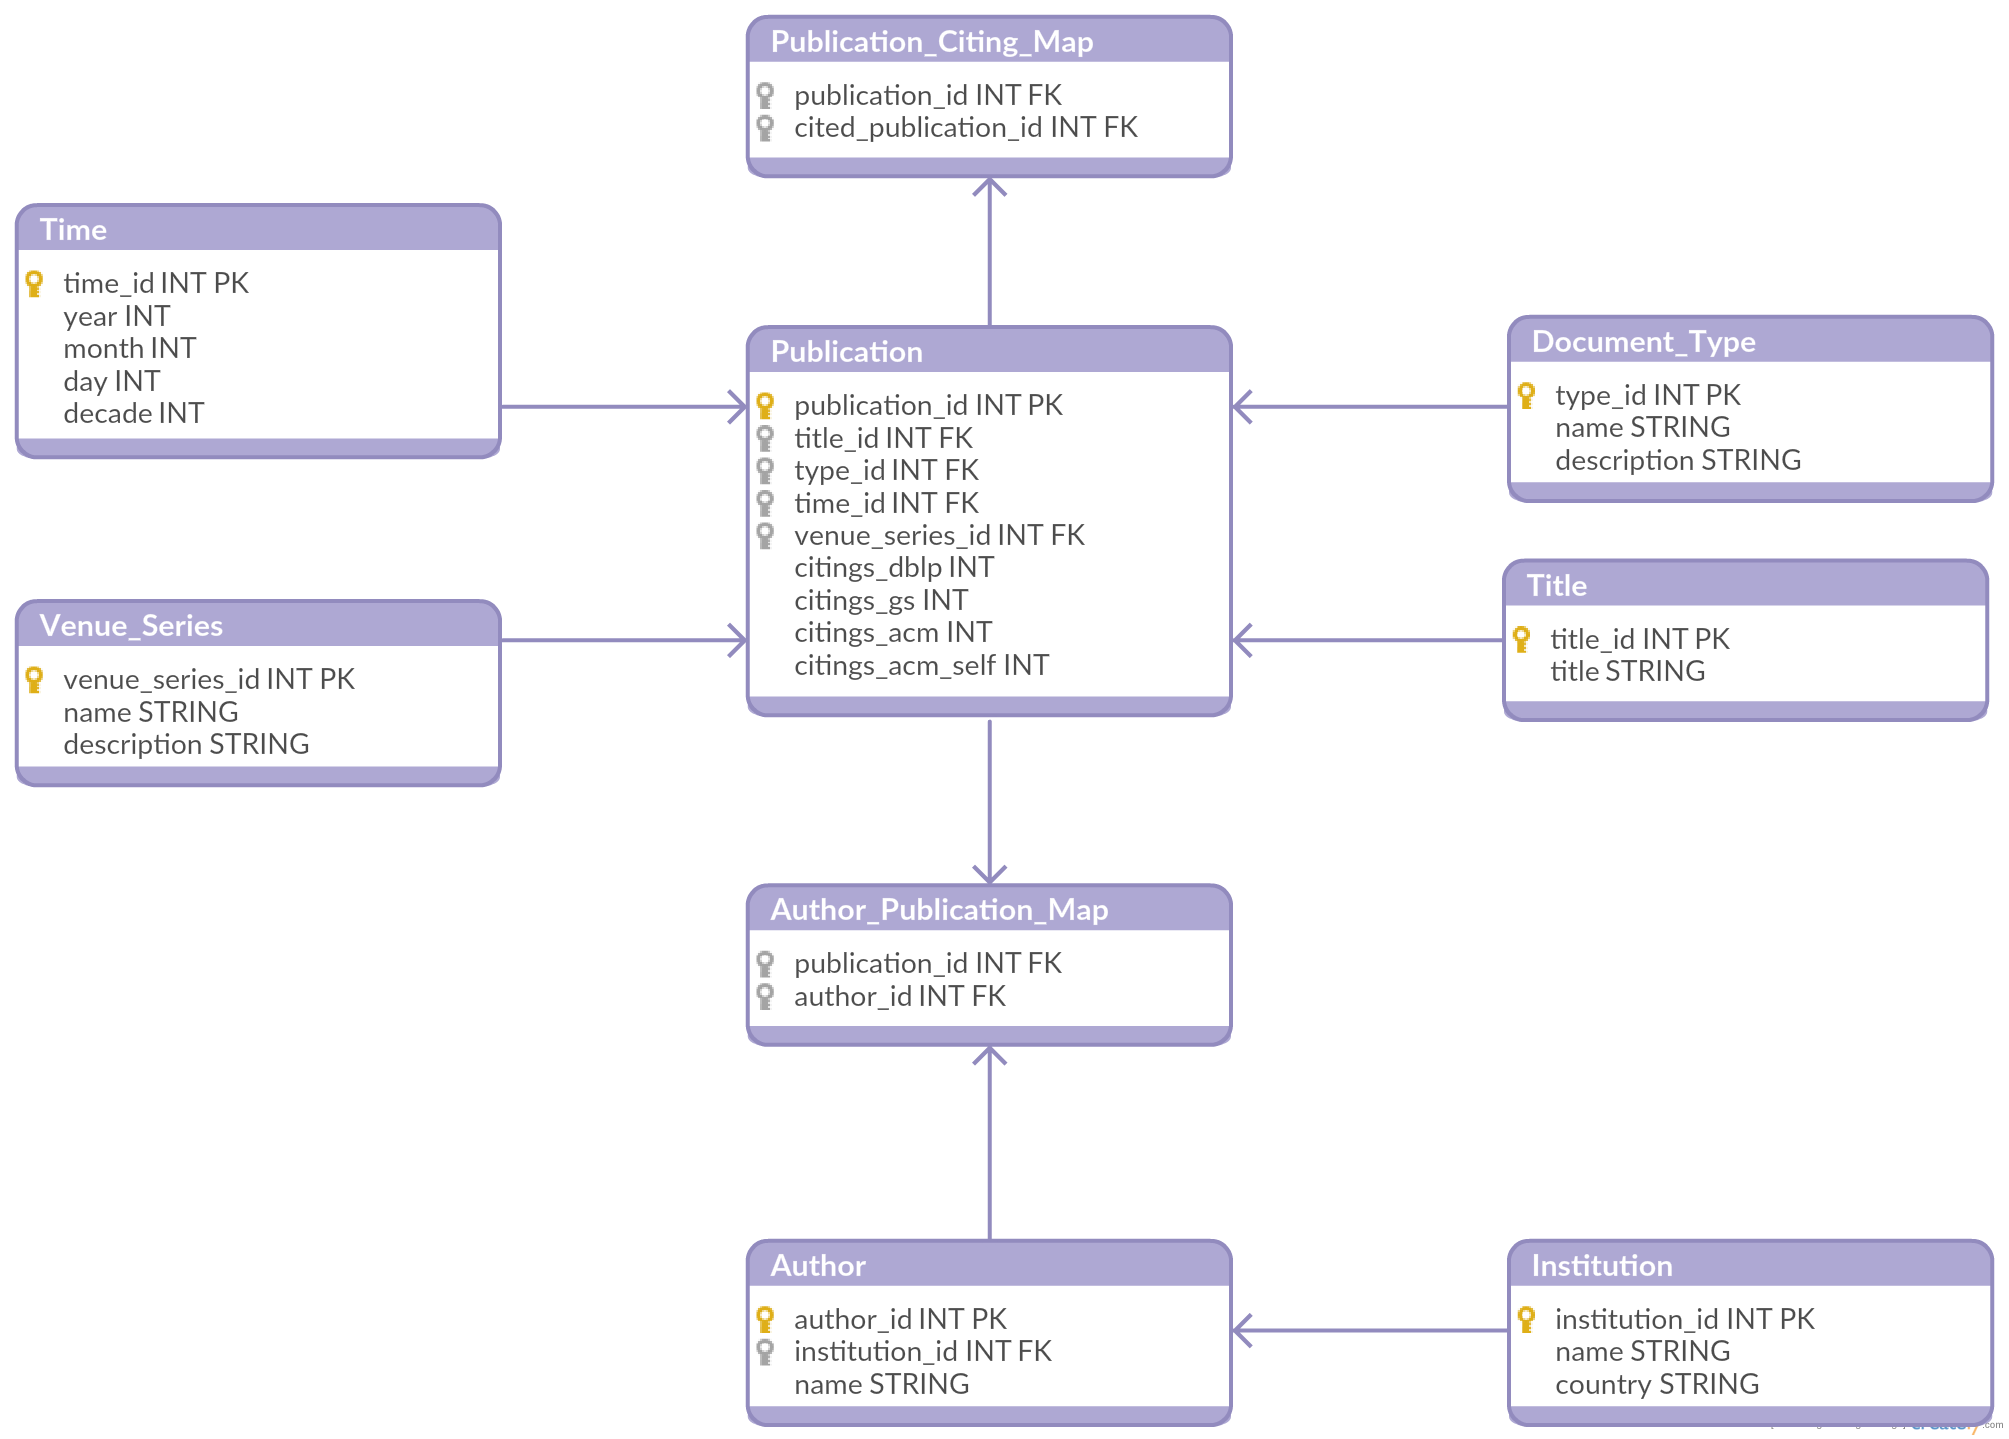
\includegraphics[width=\textwidth]{pics/schema.png}

\begin{itemize}
    \item \texttt{Publication\_Citing\_Map}: Zitat einer Publikation (nicht Teil des endgültigen Sternschemas)
    \item \texttt{Publication}: Zitierungszahlen werden aus \texttt{Publication\_Citing\_Map} generiert
    \item \texttt{Document\_Type}: Typ der Publication, z.\,B. Journal, Artikel, Kollektion
\end{itemize}

\section{Datenimport und -Transformation}

Der Import der Daten gestaltete sich aufgrund der Datengröße schwierig. So kann die \texttt{dblp.xml} nicht direkt mit einem DOM-Parser verarbeitet werden, da dafür zu viel Speicher benötigt wird. Aus diesem Grund muss ein SAX- oder StaX-Parser verwendet werden.

Auch ein direkter Import per MapReduce stellte sich als schwierig heraus, da immer komplette XML-Records gelesen werden müssen, was der standardmäßig zeilenweisen Verarbeitung von MapReduce widerspricht. Hadoop besitzt zwar einen \texttt{StreamXmlRecordReader}, der jedoch selbst in aktuellen Versionen scheinbar nicht immer problemlos funktioniert\footnote{\url{https://issues.apache.org/jira/browse/MAPREDUCE-577}}.

Alternativ wird oft \texttt{XmlInputFormat} von Mahout (einem Hadoop-basierten Machine-Learning-Tool) verwendet\footnote{\url{http://oobaloo.co.uk/articles/2010/1/20/processing-xml-in-hadoop.html}}, was diese Probleme nicht hat. Allerdings müssen dabei alle zu lesenden Records das gleiche XML-Tag verwenden, was bei der \texttt{dblp.xml} leider nicht der Fall ist.

Aus diesem Grund haben wir ein eigenes Tool für den Import entwickelt. Der \texttt{pub-importer}\footnote{\url{https://github.com/klemens/bigdata-kylin-dblp}} liest die \texttt{dblp.xml} aus einer Datei oder von \texttt{stdin}, verwendet StAX für das Parsen und schreibt das Ergebnis anschließend direkt ins HDFS. Dabei ist unabhängig von der Größe der Eingabedatei der Speicherverbrauch konstant.

Die exportierten Daten werden dabei in einem zu Hive (oder alternativ zu unserem \texttt{dblp-formatter}) kompatiblen Format geschrieben (CSV mit Backslash als Escape-Zeichen oder mit Anführungszeichen versehen) und bestehen aus zwei Dateien: Einmal die \texttt{Collections} wie Konferenzberichte oder Bücher und schließlich die \texttt{Publications} an sich mit entsprechenden Verweisen auf die \texttt{Collections}.

Zusätzlich kann der \texttt{pub-importer} auch den im Data-Warehouse-Praktikum verwendeten, unvollständigen xml-Dump von ACM lesen und auf die gleiche Weise ins HDFS schreiben. Da dort jedoch keine Informationen über die Journals enthalten sind, entfällt hierbei die \texttt{Collections}-Datei.

\subsection{Probleme bei der Datentransformation mit PDI}

Bei der Umsetzung der Datentransformation mit PDI kam es zu einigen Problemen. Ein Problem ist die Implementierung des OUTER-JOIN in PDI. Diese Implementierung arbeitet nicht wie erwartet. Dies könnte daran liegen, dass die OUTER-JOIN Logik ausschließlich als Merge-JOIN implementiert ist. Da sich dieses Problem mit einigem Aufwand umgehen lässt, ist die Umsetzung der Tranformation mit PDI daran letztlich nicht gescheitert. Dafür jedoch an den folgenden Problemen.

PDI hat bei der Umsetzung stets sämtliche Schritte (Vergleich, Sortierung, Merge, etc.) parallel im Arbeitsspeicher ausgeführt. Es war daher auch mit 12 GB RAM nicht möglich alle Transformation auf der gesamten Datenmenge durchzuführen. Nach Laufzeiten von bis zu vier Stunden war das Ergebnis immer nur eine Exception. Für kleine Datenmengen hingegen funktionierte die selbe Transformation tadellos.

Darüber hinaus stellte sich während der Umsetzung heraus, dass die in PDI designten Transformationen nicht ohne weiteres auf dem Server ausführbar sind. Diese müssen (insofern kein zusätzlicher Deployment-Prozess dafür implementiert wird) auf dem Server immer an mehreren Stellen neu konfiguriert und angepasst werden, bevor sie ausführbar sind. Je komplexer die Transformation ist, umso umfangreicher sind die nötigen Anpassungen. Zusätzlich zu diesen Einschränkungen ist es alles andere als trivial, die Ausführung der Transformationen so zu konfigurieren, dass die Vorteile eines vorhandenen Clusters vollständig ausgenutzt werden.

Aus diesen Gründen ist das Verhältnis zwischen Aufwand und Nutzen sehr schlecht. Daher wurde die Datentransformation nicht, wie ursprünglich geplant, mit PDI umgesetzt.

\subsection{Datentransformation mit Apache Flink}

Nach den Problemen mit PDI wurde die Datentransformation in das Sternschema mittels Apacha Flink implementiert, woraus dann der \texttt{dblp-formatter} entstand.

Allerdings gab es auch hier einige Komplikationen: Das Problem ist die Verwendung von zwei verschiedenen CSV-Implementierungen, einmal der CSVReader von Apache Commons und dann der CSVReader von Apache Flink, wobei sich letzterer an keinerlei Standards (RFC 4180) hält und sich auch nicht ausreichend konfigurieren lässt. So unterstützt er nur die Quoting-Variante zum Speichern von CSVs. Allerdings erwartet er nicht wie üblich eine Verdopplung des Quoting-Zeichens, wenn dieses innerhalb eines Strings auftaucht, sondern erwartet das Escaping des Quoting-Zeichens mit einem Backslash, was weder dem Standard entspricht, noch mit dem CSVWriter von Apache Commons ausgegeben werden kann.

Abgesehen von diesem Problem läuft der Transformationsvorgang reibungslos. So werden zuerst die Dimensionstabellen erzeugt, indem die nötigen Felder aus den importierten Dateien in neue CSV-Dateien projiziert werden. Jeder Eintrag in den Tabellen ist dabei eindeutig. Die Faktentabelle entsteht anschließend durch einen Join der Dimensionstabellen. Der gesamte Vorgang dauert auf den dblp-Daten ca. zehn Minuten.

\subsection{Externe Hive-Tabellen}

Nach Abschluss des Datenverarbeitungsschrittes, bei dem die Daten mit dem \texttt{dblp-formatter} in einzelne CSV-Dateien überführt werden, wurden darauf externe Hive-Tabellen definiert, um den Zugriff aus Kylin zu ermöglichen.

\section{Analyse}
\label{sec:Analyse}

\subsection{Cube-Generierung mit Kylin}

Die Cube-Generierung erfolgt mittels des durch Kylin verfügbaren Webinterface unter der URL \url{http://localhost:7070/kylin}. Es wurden im Verlauf des Praktikums mehrere Projekte mit verschiedenen Inhalten in Kylin angelegt. In jedem Projekt mussten als Grundlage zur Cube-Erzeugung die benötigten Tabellen aus Hive importiert werden. Anschließend wurde der Cube zur Datenanalyse erzeugt. Die Cubes wurden so entworfen, dass sie möglichst umfangreiche Analysen zulassen. Nach der Cube Konfiguration wurde dieser über einen zugehörigen Job gebaut. Dies dauerte ca. 80 Minuten und wurde durch von Kylin erzeugte Map-Reduce-Jobs umgesetzt. Der erzeugte Cube ist dann in HBASE persistiert. Sobald dieser Punkt erreicht ist, kann über das Query-Interface von Kylin (basierend auf Apache Calcite) auf die Daten des Cubes zugegriffen werden. 

\subsection{Analyse der Daten aus den Cubes}

Im Projekt lag der Schwerpunkt bei der Analyse der Daten nicht auf den Ergebnissen der einzelnen Abfragen sondern auf dem Vergleich der Ausführungszeiten der Abfragen a) basierend auf den in Kylin erzeugten Cubes und b) direkt auf den Tabellen in Hive. Es wurden verschiedene Abfragen entworfen, die bei Ausführung auf dem Cube in Kylin und auch direkt auf den Hive Tabellen die gleichen Ergebnisse liefern. Diese Abfragen sind im Webinterface von Kylin im Bereich "Query" als \glqq gespeicherte Queries\grqq{} hinterlegt. Die Abfragen müssen zur Verwendung in der Hive Shell allerdings teilweise modifiziert werden, da der Funktionsumfang des auf Apache Calcite basierenden Query Interface von Kylin und der Hive Shell unterschiedlich ist.

\section{Ergebnisse}
\label{sec:Ergebnisse}

Die Analyse der DBLP Daten ergab, dass diese für eine Zitationsanalyse ungeeignet sind. Die DBLP Daten enthalten prinzipiell nur wenige Verweise zu Zitierungen. Darüber hinaus sind die vorhandenen Verweise (verglichen mit Google Scholar) unvollständig. Zusätzlich wurde deutlich, dass die DBLP Daten für ältere Publikationen (vor 2000 publiziert) qualitativ und quantitativ deutlich besser erfasst sind, als für aktuellere. Im Bezug auf die Analyse von Zitierungen wäre es daher interessant zukünftig z.B. Google Scholar als Datenquelle zu verwenden.\medskip\par

\noindent Hinsichtlich der Ausführungszeiten einzelner Abfragen ergab sich eine deutliche Beschleunigung bei Verwendung der mit Kylin erzeugten Cubes im Vergleich zu den Ausführungszeiten bei direkter Verwendung der Hive Tabellen über die Hive Shell. Die in der Abschlusspräsentation dargestellten Werte sind jedoch nur als grober Identifikator für die Verbesserung der Performance bzgl. der Ausführungszeit der einzelnen Abfragen zu verstehen. Hier gibt es sowohl in Kylin, als auch in Hive mehrere Optimierungsmöglichkeiten, welche einen Einfluss auf die erhaltenen Messwerte haben können.

\subsection{Fazit}

Abschließend kann festgehalten werden, dass alle im Projekt verwendeten Technologien durchaus ihre Daseinsberechtigung haben. Es gibt jedoch bei allen Tools noch den ein oder anderen Bug, den es im Verlauf der Umsetzung zu beheben gilt. Die Auswertung der Ergebnisse zeigt, dass Kylin die Analyse der Daten deutlich beschleunigen kann. Allerdings gibt es noch einige Konfigurationsmöglichkeiten, die Einfluss auf die in Kylin oder Hive erreichbaren Werte haben können. Die Betrachtung dieser noch ungenutzten Möglichkeiten, sowie ein Vergleich von Kylin mit einer ähnlichen Technologie wie z.B. Cloudera Impala, stellen spannende Aufgaben für die Zukunft dar.

\end{document}
